\documentclass[10pt,twocolumn]{article}

\usepackage[T1]{fontenc}
\usepackage{lmodern}
\usepackage[margin=0.62in,columnsep=0.24in]{geometry}
\usepackage{amsmath,amssymb,mathtools,bm}
\usepackage{booktabs,enumitem}
\usepackage{xcolor,graphicx,microtype}
\usepackage{tikz}
\usetikzlibrary{arrows.meta,positioning,calc,decorations.pathreplacing}
\usepackage[colorlinks=true,linkcolor=blue!45!black,
  citecolor=blue!45!black,urlcolor=blue!45!black]{hyperref}
\usepackage{fancyhdr}

\setlength{\parindent}{0.9em}
\setlength{\parskip}{0pt}
\setlength{\abovedisplayskip}{5pt}
\setlength{\belowdisplayskip}{5pt}
\setlength{\abovedisplayshortskip}{3pt}
\setlength{\belowdisplayshortskip}{3pt}
\setlength{\tabcolsep}{3.0pt}
\renewcommand{\arraystretch}{1.08}
\raggedbottom

\pagestyle{fancy}
\fancyhf{}
\fancyhead[L]{\footnotesize Molecular-vibronic H$_2$O}
\fancyhead[R]{\footnotesize Materials computation}
\fancyfoot[C]{\thepage}
\renewcommand{\headrulewidth}{0.25pt}

\newcommand{\ket}[1]{\lvert #1\rangle}
\newcommand{\bra}[1]{\langle #1\rvert}
\newcommand{\braket}[2]{\langle #1\mid #2\rangle}
\newcommand{\Ha}{\mathrm{Ha}}
\newcommand{\bohr}{a_0}
\newcommand{\R}{\mathbb R}
\newcommand{\C}{\mathbb C}
\newcommand{\Tr}{\operatorname{Tr}}
\newcommand{\Span}{\operatorname{span}}
\newcommand{\conceptbreak}{%
  \par\medskip\noindent
  {\color{black!30}\rule{\columnwidth}{0.35pt}}%
  \par\medskip}
\newcommand{\micro}{\paragraph{Micro-intuition.}}
\newcommand{\mathderiv}{\paragraph{Mathematical construction.}}
\newcommand{\commentaryblock}{\paragraph{Commentary.}}
\newcommand{\physical}{\paragraph{Physical interpretation.}}
\newcommand{\materials}{\paragraph{Materials-science interpretation.}}
\newcommand{\impl}{\paragraph{Implementation translation.}}
\newcommand{\audit}{\paragraph{Audit checkpoint.}}
\newcommand{\codeword}[1]{\texttt{\detokenize{#1}}}
\newcommand{\codepath}[1]{\nolinkurl{#1}}

\title{From First-Principles Electronic Structure to a\
Molecular-Vibronic H$_2$O Hamiltonian\\
\large A Self-Contained Materials-Science and Molecular-Physics Primer}
\author{Jake Skyler Strobel\\University of Wisconsin--Madison}
\date{17 July 2026}

\begin{document}
\maketitle
\vspace{-1.45em}

\begin{abstract}
This primer constructs the current molecular-vibronic H$_2$O model from its
physical starting point to its coupled electronic--vibrational eigenproblem.
Nuclei and electrons first enter through their Coulomb Hamiltonian.  Fixing the
nuclei defines a Born--Oppenheimer electronic surface, and a restricted
Hartree--Fock calculation in an STO-3G Gaussian basis supplies an equilibrium
geometry, molecular orbitals, electronic integrals, gradient, and Hessian.
Mass weighting diagonalizes the Hessian into bend, symmetric-stretch, and
antisymmetric-stretch coordinates.  Freezing the oxygen core and retaining a
CAS$(8e,6o)$ orbital space then defines the correlated electronic degrees of
freedom.  Centered, orbital-aligned finite differences construct the scalar,
one-electron, and two-electron response of that Hamiltonian along each normal
coordinate.  Quantizing those coordinates produces explicit
electron--vibration interactions, including the two-electron response
$a^\dagger a^\dagger(b^\dagger+b)aa$.  The coupled Hamiltonian is finally
diagonalized in an electronic-configuration times vibrational-occupation
basis.  The development emphasizes the derivations and physical mechanisms
that determine this model, then closes with materials-style convergence,
matched-geometry cross-code validation, and the precise limitations of the
present orbital basis, electronic surface, linear expansion, and vibrational
cutoff.
\end{abstract}

\section*{The complete object-and-map architecture}

The calculation is one composition of typed physical and numerical maps:
{\scriptsize
\begin{equation}
\begin{aligned}
\{Z_A,M_A,\mathbf R_A\}
&\xmapsto{\text{Coulomb model}}\hat H(\mathbf r,\mathbf R),\\
\hat H(\mathbf r,\mathbf R)
&\xmapsto{\text{BO surface}}U_0(\mathbf R),\\
U_0(\mathbf R)
&\xmapsto{\text{RHF/STO-3G}}(\mathbf R_0,C,h,g,K),\\
K&\xmapsto{M^{-1/2}KM^{-1/2}}(\omega_\mu,L_\mu),\\
(h,g,L_\mu)&\xmapsto{\text{CAS + finite difference}}
(\hat H_{\rm el}^{(0)},\hat D_\mu),\\
(\hat H_{\rm el}^{(0)},\hat D_\mu,\omega_\mu)
&\xmapsto{\text{quantize }Q_\mu}\hat H_{\rm vib},\\
\hat H_{\rm vib}
&\xmapsto{\text{configuration basis}}H_{\mathcal B},\\
H_{\mathcal B}
&\xmapsto{\text{sparse eigensolve}}(E_0,\ket{\Psi_0}).
\end{aligned}
\label{eq:architecture}
\end{equation}}
Here $A$ labels nuclei, $Z_A$ is nuclear charge, $M_A$ is nuclear mass,
$\mathbf R_A$ is nuclear position, $\mathbf r$ denotes all electron
coordinates, $U_0$ is the ground electronic potential-energy surface,
$\mathbf R_0$ is its computed equilibrium geometry, $C$ is the molecular-
orbital coefficient matrix, $h$ and $g$ are one- and two-electron integral
tensors, $K$ is the Cartesian Hessian, $L_\mu$ is normal mode $\mu$, and
$\omega_\mu$ is its harmonic frequency.  The active electronic Hamiltonian
$\hat H_{\rm el}^{(0)}$ and its derivative $\hat D_\mu$ become the coupled
molecular-vibronic Hamiltonian $\hat H_{\rm vib}$.  The basis
$\mathcal B=\{\ket I_{\rm el}\otimes\ket{\mathbf n}_{\rm vib}\}$ combines
electronic configurations $I$ with vibrational occupations
$\mathbf n=(n_b,n_s,n_a)$.  Matrix representation in this basis gives
$H_{\mathcal B}$, whose lowest eigenpair is $(E_0,\ket{\Psi_0})$.

\begin{center}
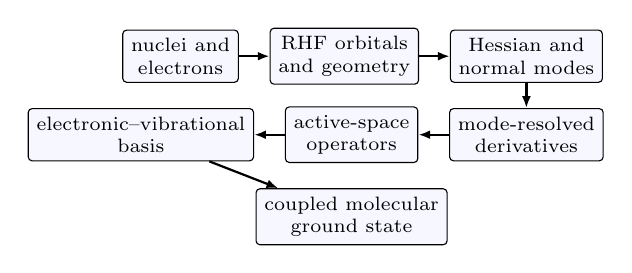
\begin{tikzpicture}[
  node distance=3.2mm and 3.9mm,
  every node/.style={font=\scriptsize,align=center},
  box/.style={draw,rounded corners=1.4pt,inner sep=3pt,fill=blue!3},
  arr/.style={-{Latex[length=1.5mm]},thick}
]
\node[box] (matter) {nuclei and\\electrons};
\node[box,right=of matter] (scf) {RHF orbitals\\and geometry};
\node[box,right=of scf] (modes) {Hessian and\\normal modes};
\node[box,below=of modes] (fd) {mode-resolved\\derivatives};
\node[box,left=of fd] (second) {active-space\\operators};
\node[box,left=of second] (basis) {electronic--vibrational\\basis};
\node[box,below=of second] (solve) {coupled molecular\\ground state};
\draw[arr] (matter)--(scf);
\draw[arr] (scf)--(modes);
\draw[arr] (modes)--(fd);
\draw[arr] (fd)--(second);
\draw[arr] (second)--(basis);
\draw[arr] (basis)--(solve);
\end{tikzpicture}
\end{center}

\materials The architecture resembles a standard first-principles materials
workflow because each stage turns a microscopic model into a more directly
computable representation, and each representation has its own convergence
control.  A crystal calculation may converge plane-wave cutoff and Brillouin-
zone sampling.  This finite molecule instead requires an orbital-basis study,
an active-space study, finite-difference checks, a vibrational cutoff study,
and a solver check.  Both workflows express the same scientific discipline:
state the representation, converge it, validate it, and preserve the map from
raw calculation to reported observable.

\conceptbreak

\section*{Part I. The molecular quantum problem}

\subsection*{Nuclei and electrons}

\micro Water is a three-nucleus, ten-electron Coulomb system.  Its geometry
and vibrations arise from the same electronic and nuclear interactions that
determine its ground-state energy.

\mathderiv In atomic units, where $\hbar=e=m_e=4\pi\epsilon_0=1$, the
nonrelativistic molecular Hamiltonian is
\begin{align}
\hat H={}&-\sum_{i=1}^{N_e}\frac12\nabla_i^2
-\sum_{A=1}^{N_N}\frac{1}{2M_A}\nabla_A^2
-\sum_{iA}\frac{Z_A}{|\mathbf r_i-\mathbf R_A|}\nonumber\\
&+\sum_{i<j}\frac{1}{|\mathbf r_i-\mathbf r_j|}
+\sum_{A<B}\frac{Z_AZ_B}{|\mathbf R_A-\mathbf R_B|}.
\label{eq:full-coulomb}
\end{align}
This Hamiltonian and its Born--Oppenheimer reduction are standard molecular
quantum-mechanics constructions \cite{BornOppenheimer,SzaboOstlund}.
The index $i$ labels electrons, $A$ labels nuclei, $N_e=10$ for neutral
H$_2$O, and $N_N=3$.  The Laplacians $\nabla_i^2$ and $\nabla_A^2$ generate
electronic and nuclear kinetic energies.  The remaining terms are electron--
nucleus attraction, electron--electron repulsion, and nucleus--nucleus
repulsion.  The exact wavefunction
$\Psi(\mathbf r_1s_1,\ldots,\mathbf r_{N_e}s_{N_e};\mathbf R_1,\ldots)$
depends on every electron position $\mathbf r_i$, spin $s_i$, and nuclear
position $\mathbf R_A$.

\commentaryblock Equation~\eqref{eq:full-coulomb} is the common microscopic
starting point for molecular quantum chemistry and electronic-structure
materials science.  The complexity comes from the pair interaction
$|\mathbf r_i-\mathbf r_j|^{-1}$: one electron moves in a field that depends on
all other electron positions, so a product of independent one-electron
solutions cannot represent the exact state.

\subsection*{Born--Oppenheimer separation}

\micro Nuclei are thousands of times heavier than electrons.  Electronic
motion can therefore be solved at a sequence of fixed nuclear geometries, and
the resulting electronic energy acts as a potential for nuclear motion.

\mathderiv For fixed nuclear coordinates $\mathbf R$, define the clamped-
nuclei electronic Hamiltonian
\begin{align}
\hat H_{\rm el}(\mathbf R)
={}&-\sum_i\frac12\nabla_i^2
-\sum_{iA}\frac{Z_A}{|\mathbf r_i-\mathbf R_A|}
+\sum_{i<j}\frac{1}{|\mathbf r_i-\mathbf r_j|}\nonumber\\
&+V_{NN}(\mathbf R),
\qquad
V_{NN}=\sum_{A<B}\frac{Z_AZ_B}{R_{AB}}.
\label{eq:clamped}
\end{align}
Its eigenproblem is
\begin{equation}
\hat H_{\rm el}(\mathbf R)\psi_k(\mathbf r;\mathbf R)
=U_k(\mathbf R)\psi_k(\mathbf r;\mathbf R).
\label{eq:bo-surface}
\end{equation}
The scalar function $U_k(\mathbf R)$ is a potential-energy surface.  Nuclear
motion on the ground surface obeys, within the Born--Oppenheimer
approximation,
\begin{equation}
\left[-\sum_A\frac{\nabla_A^2}{2M_A}+U_0(\mathbf R)\right]
\chi_\nu(\mathbf R)=\mathcal E_\nu\chi_\nu(\mathbf R).
\label{eq:nuclear-schrodinger}
\end{equation}
Here $\chi_\nu$ is a nuclear vibrational wavefunction and $\mathcal E_\nu$ is
a molecular rovibrational energy after rotational treatment is specified.

\physical An equilibrium structure is a local minimum of $U_0$.  A vibrational
frequency measures the local curvature of $U_0$ around that minimum.  A
vibronic coupling measures how the electronic Hamiltonian itself changes as a
nucleus moves along a collective vibrational direction.  Geometry, frequency,
and coupling are therefore three levels of information extracted from one
electronic surface.

\conceptbreak

\section*{Part II. RHF/STO-3G electronic structure}

\subsection*{From continuous orbitals to a finite basis}

\micro A basis set replaces each unknown continuous molecular orbital by a
finite linear combination of known atom-centered functions.

\mathderiv A primitive Cartesian Gaussian centered on nucleus $A$ has the form
\begin{align}
g_{\alpha\ell mn}(\mathbf r-\mathbf R_A)
={}&N(x-X_A)^\ell(y-Y_A)^m\nonumber\\
&\times(z-Z_A)^n e^{-\alpha|\mathbf r-\mathbf R_A|^2},
\label{eq:primitive-gaussian}
\end{align}
where $\alpha>0$ is the exponent, $(\ell,m,n)$ selects angular character, and
$N$ normalizes the function.  A contracted STO-3G atomic orbital is
\begin{equation}
\chi_\mu(\mathbf r)=\sum_{k=1}^{3}d_{\mu k}g_{\alpha_{\mu k}}(\mathbf r),
\label{eq:sto3g}
\end{equation}
where the three primitive Gaussians approximate the radial shape of one
Slater-type atomic orbital \cite{STO3G}.  Molecular orbital $p$ is expanded as
\begin{equation}
\phi_p(\mathbf r)=\sum_{\mu=1}^{N_{\rm AO}}C_{\mu p}\chi_\mu(\mathbf r).
\label{eq:lcaomo}
\end{equation}
The overlap matrix $S_{\mu\nu}=\langle\chi_\mu|\chi_\nu\rangle$ appears because
atom-centered Gaussians are generally nonorthogonal.

In the minimal water basis, oxygen contributes functions with $1s$, $2s$, and
three $2p$ characters; each hydrogen contributes one $1s$ function.  The
resulting seven-dimensional AO space is the finite coordinate system in which
the classical electronic problem is assembled.

\mathderiv Positive-definite $S$ admits the spectral factorization
\begin{equation}
S=U s U^{\mathsf T},\qquad
X=S^{-1/2}=U s^{-1/2}U^{\mathsf T}.
\label{eq:symmetric-orthogonalization}
\end{equation}
The transformed basis has overlap $X^{\mathsf T}SX=I$.  Consequently, a
generalized eigenproblem can be solved as an ordinary symmetric problem:
\begin{equation}
F'=X^{\mathsf T}FX,\qquad
F'C'=C'\varepsilon,\qquad C=XC'.
\label{eq:orthogonalized-fock}
\end{equation}

\commentaryblock ``STO-3G'' names the electronic orbital basis.  Three
primitive Gaussians build each contracted atomic function, and seven such
functions span the molecular orbitals of water.  The later vibrational
occupation basis resolves nuclear motion in a different Hilbert space.
Basis-set convergence enlarges the electronic space with additional radial and
angular functions; vibrational convergence enlarges the nuclear space with
additional oscillator levels.

\subsection*{Restricted Hartree--Fock and self-consistency}

\micro RHF represents a closed-shell singlet by one Slater determinant whose
spatial orbitals are occupied by paired alpha and beta electrons.

\mathderiv Let $\{\varphi_i\}_{i=1}^{N_e}$ be orthonormal spin orbitals.  Their
antisymmetric determinant is
\begin{equation}
\Phi_{\rm RHF}(x_1,\ldots,x_{N_e})
=\frac{1}{\sqrt{N_e!}}\det[\varphi_i(x_j)],
\label{eq:slater}
\end{equation}
where $x_j=(\mathbf r_j,s_j)$ includes position and spin.  Antisymmetry under
exchange supplies Fermi statistics.  Let $C_o$ collect the occupied spatial
orbitals.  Their orthonormality constraint is $C_o^{\mathsf T}SC_o=I$.
Introduce the Lagrangian
\begin{equation}
\mathcal L(C_o,\varepsilon)
=E_{\rm RHF}[C_o]
-2\Tr\!\left[\varepsilon(C_o^{\mathsf T}SC_o-I)\right].
\label{eq:rhf-lagrangian}
\end{equation}
Variation with respect to $C_o$ gives the Roothaan--Hall equation
\begin{equation}
\frac{\partial\mathcal L}{\partial C_o}=0
\quad\Longrightarrow\quad
FC_o=SC_o\varepsilon.
\label{eq:roothaan}
\end{equation}
This finite-basis Hartree--Fock equation was introduced by Roothaan
\cite{Roothaan} and is derived in standard quantum-chemistry treatments
\cite{SzaboOstlund}.
The matrix $F$ is the Fock operator, $C$ contains the MO coefficients,
$S$ is the AO overlap matrix, and diagonal $\varepsilon$ contains orbital
energies.  For a closed shell, the AO density and Fock matrices are
\begin{align}
P_{\mu\nu}&=2\sum_{i\in\mathrm{occ}}C_{\mu i}C_{\nu i},
\label{eq:density}\\
F_{\mu\nu}&=h^{\rm core}_{\mu\nu}
+\sum_{\lambda\sigma}P_{\lambda\sigma}
\left[(\mu\nu|\lambda\sigma)-\frac12(\mu\lambda|\nu\sigma)\right].
\label{eq:fock}
\end{align}
The one-electron matrix $h^{\rm core}$ contains electronic kinetic energy and
electron--nucleus attraction.  The electron-repulsion integral is
\begin{equation}
(\mu\nu|\lambda\sigma)=
\iint\frac{\chi_\mu(\mathbf r_1)\chi_\nu(\mathbf r_1)
\chi_\lambda(\mathbf r_2)\chi_\sigma(\mathbf r_2)}
{r_{12}}\,d\mathbf r_1d\mathbf r_2.
\label{eq:ao-eri}
\end{equation}
Before SCF begins, the integral engine evaluates the overlap $S$, kinetic
energy $T$, nuclear-attraction matrix $V$, and four-index electron-repulsion
tensor.  Their one-electron combination is
\begin{equation}
h^{\rm core}=T+V.
\label{eq:core-integrals}
\end{equation}
Gaussians are computationally effective because the product of two $s$-type
primitives is another Gaussian centered between the original nuclei:
\begin{align}
e^{-\alpha|\mathbf r-\mathbf A|^2}
e^{-\beta|\mathbf r-\mathbf B|^2}
={}&e^{-\frac{\alpha\beta}{\alpha+\beta}|\mathbf A-\mathbf B|^2}
e^{-(\alpha+\beta)|\mathbf r-\mathbf P|^2},\nonumber\\
\mathbf P={}&\frac{\alpha\mathbf A+\beta\mathbf B}{\alpha+\beta}.
\label{eq:gaussian-product}
\end{align}
The Gaussian product theorem reduces multicenter integrals to reusable
one-center recurrence relations.  Angular factors generate families of
integrals from lower-angular-momentum quantities, and contraction coefficients
combine primitive results into the STO-3G matrix elements.  This is the
classical numerical machinery hidden beneath the compact symbols $S$, $h$, and
$(\mu\nu|\lambda\sigma)$.

These arrays are the numerical representation of the continuous Coulomb
operator.  The four-index tensor is the expensive object: its formal storage
grows as $N_{\rm AO}^4$, and its repeated contraction with $P$ builds the
Coulomb and exchange contribution to $F$.  The present PK algorithm stores and
contracts these integrals directly, which is practical for the seven-function
STO-3G calculation.

Equations~\eqref{eq:density}--\eqref{eq:fock} are solved iteratively: a trial
density builds $F$, Eq.~\eqref{eq:roothaan} gives new orbitals, and those
orbitals give a new density.  A useful stationarity residual is the AO
commutator
\begin{equation}
R_{\rm SCF}=FPS-SPF.
\label{eq:scf-residual}
\end{equation}
At self-consistency, the occupied subspace diagonalizes its own Fock operator,
so $R_{\rm SCF}$ vanishes.  Practical SCF codes monitor changes in energy and
density together with this residual; direct inversion in the iterative
subspace (DIIS) combines previous residuals to accelerate convergence.  The
converged RHF energy is
\begin{equation}
E_{\rm RHF}=V_{NN}+\frac12\sum_{\mu\nu}P_{\mu\nu}
\left(h^{\rm core}_{\mu\nu}+F_{\mu\nu}\right).
\label{eq:rhf-energy}
\end{equation}

\commentaryblock A practical SCF calculation begins from an orbital guess,
often obtained by diagonalizing the core Hamiltonian or superposing atomic
densities.  Each cycle performs the map
\begin{equation}
P^{(k)}\longmapsto F[P^{(k)}]
\longmapsto C^{(k+1)}\longmapsto P^{(k+1)}.
\label{eq:scf-map}
\end{equation}
Simple fixed-point iteration can oscillate because the Coulomb and exchange
fields change with the orbitals they determine.  DIIS stores several recent
Fock matrices and residuals, then chooses coefficients that minimize an
extrapolated commutator residual subject to their sum being one.  Damping and
level shifting are complementary stabilizers when early iterations change too
aggressively.  Convergence requires simultaneous agreement of energy, density,
and stationarity residual; a small energy change alone can hide a rotating
occupied subspace.

Canonical RHF orbitals diagonalize the converged Fock matrix.  Their individual
shapes and orbital energies help interpret bonding and antibonding character,
yet rotations among occupied orbitals leave the determinant and total energy
unchanged.  The occupied projector, density, total energy, and expectation
values are consequently more invariant objects than any single orbital plot.

\impl The current fixture uses Psi4 1.10.2 with SCF/RHF, the PK integral
algorithm, and STO-3G.  Psi4 solves Eq.~\eqref{eq:roothaan}, evaluates analytic
gradients and a Hessian, and supplies AO/MO integral tensors at the center and
displaced geometries \cite{Psi4}.

\subsection*{Geometry optimization}

\micro Geometry optimization converts repeated electronic ground-state
solutions into a search for the stationary nuclear structure.

\mathderiv The optimized geometry is the numerical solution of
\begin{equation}
\mathbf R_0=\operatorname*{arg\,min}_{\mathbf R}E_{\rm RHF}(\mathbf R),
\qquad
\nabla_{\mathbf R}E_{\rm RHF}(\mathbf R_0)\simeq\mathbf0.
\label{eq:geometry-opt}
\end{equation}
If $g_k=\nabla_{\mathbf R}E(\mathbf R_k)$ and $B_k$ approximates the nuclear
Hessian, a Newton-like step solves
\begin{equation}
B_k\Delta\mathbf R_k=-g_k,\qquad
\mathbf R_{k+1}=\mathbf R_k+\Delta\mathbf R_k.
\label{eq:geometry-step}
\end{equation}
Line searches, trust controls, or quasi-Newton updates regulate this local
quadratic model.  Every trial geometry requires a converged SCF calculation
because the nuclear gradient belongs to the self-consistent electronic state.
The retained RHF/STO-3G minimum has two equal O--H bonds of approximately
$0.990$ \AA\ and an H--O--H angle of approximately $100.0^\circ$.

\subsection*{Analytic forces and the moving AO basis}

\micro Moving a nucleus changes the nuclear repulsion, the molecular
integrals, and the atom-centered basis functions themselves.  A correct force
contains all three responses.

\mathderiv For a nuclear coordinate $R_A$, the stationary RHF Lagrangian gives
a gradient with the schematic AO form
\begin{align}
\frac{dE_{\rm RHF}}{dR_A}={}&\frac{dV_{NN}}{dR_A}
+\sum_{\mu\nu}P_{\mu\nu}h^{A}_{\mu\nu}
+\frac12\sum_{\mu\nu\lambda\sigma}
\Gamma_{\mu\nu\lambda\sigma}
(\mu\nu|\lambda\sigma)^{A}\nonumber\\
&-\sum_{\mu\nu}X_{\mu\nu}S^{A}_{\mu\nu}.
\label{eq:analytic-gradient}
\end{align}
Here a superscript $A$ denotes an integral derivative with respect to $R_A$,
$\Gamma$ is the RHF two-particle density implied by $P$, and $X$ is the
energy-weighted density that enforces orbital orthonormality.  The final term
is the Pulay contribution: as an atom moves, its Gaussian basis moves, so the
overlap matrix changes.  RHF stationarity absorbs the explicit first-order
response of optimized orbital coefficients, while the overlap response
remains in the force.

\physical The force on nucleus $A$ is
$\mathbf F_A=-\nabla_AE$.  The first term in
Eq.~\eqref{eq:analytic-gradient} is the classical nuclear repulsion response;
the middle terms measure how one- and two-electron integrals change; and the
Pulay term corrects for the geometry-dependent coordinate system used to
represent the orbitals.  Retaining this last term keeps the force consistent
with a finite, atom-centered Gaussian basis.

\physical The calculated equilibrium geometry belongs to a declared model:
RHF/STO-3G.  Experimental geometry and higher-level electronic-structure
geometries answer related questions with different approximations.  Comparing
energies or frequencies across codes therefore requires the same geometry,
basis, masses, and numerical conventions.

\conceptbreak

\section*{Part III. Hessian and normal coordinates}

\subsection*{Curvature of the molecular energy surface}

\micro A gradient gives the local slope of an energy surface.  A Hessian gives
its local curvature and therefore the restoring force for a small displacement.

\mathderiv Write the Cartesian displacement of nucleus $A$ in direction
$\alpha\in\{x,y,z\}$ as $\Delta R_{A\alpha}=R_{A\alpha}-R_{0,A\alpha}$.
The Taylor expansion about equilibrium is
\begin{align}
U_0(\mathbf R_0+\Delta\mathbf R)
={}&U_0(\mathbf R_0)\nonumber\\
&+\frac12\sum_{A\alpha,B\beta}
K_{A\alpha,B\beta}\nonumber\\
&\hspace{2.4em}\times\Delta R_{A\alpha}\Delta R_{B\beta}
+O(\Delta R^3),
\label{eq:hessian-expansion}
\end{align}
where the Cartesian Hessian is
\begin{equation}
K_{A\alpha,B\beta}=
\left.\frac{\partial^2U_0}
{\partial R_{A\alpha}\partial R_{B\beta}}\right|_{\mathbf R_0}.
\label{eq:cart-hessian}
\end{equation}
Computing $K$ differentiates the electronic gradient once more.  At second
order, the response of the self-consistent orbitals contributes explicitly.
Coupled-perturbed Hartree--Fock equations determine the first-order
occupied--virtual rotations induced by each Cartesian displacement.  Those
orbital responses combine with first- and second-derivative AO integrals,
overlap derivatives, and nuclear-repulsion derivatives to form the symmetric
Cartesian Hessian.  A finite-difference Hessian can alternatively difference
analytic gradients, trading repeated displaced calculations for a simpler
implementation.  In either route, a poorly converged SCF solution contaminates
curvature more strongly than energy because differentiation amplifies residual
noise.

\audit A true minimum has positive curvature in every internal coordinate.
Negative eigenvalues of the internal mass-weighted Hessian correspond to
imaginary harmonic frequencies and signal a saddle point or an unconverged
electronic/geometry calculation.  Six near-zero rigid-body eigenvalues are
expected for an isolated nonlinear molecule before projection; their size is a
diagnostic of translation invariance, rotation invariance, and numerical
precision.

Mass-weighted displacements and the mass-weighted Hessian are
\begin{equation}
x_{A\alpha}=\sqrt{M_A}\,\Delta R_{A\alpha},
\qquad
F_{A\alpha,B\beta}=
\frac{K_{A\alpha,B\beta}}{\sqrt{M_AM_B}}.
\label{eq:mass-weight}
\end{equation}
After translation and rotation are projected out, solve
\begin{equation}
F L_\mu=\omega_\mu^2L_\mu,
\qquad L_\mu^{\mathsf T}L_\nu=\delta_{\mu\nu}.
\label{eq:normal-eigenproblem}
\end{equation}
The normal coordinate $Q_\mu$ is defined by
\begin{equation}
x_{A\alpha}=\sum_\mu L_{A\alpha,\mu}Q_\mu,
\qquad
\Delta R_{A\alpha}=\sum_\mu
\frac{L_{A\alpha,\mu}}{\sqrt{M_A}}Q_\mu.
\label{eq:normal-transform}
\end{equation}
Thus one scalar $Q_\mu$ moves all three nuclei in the collective pattern
$L_\mu$.

\mathderiv Collect the mode vectors as columns of $L$ and write
$\mathbf x=L\mathbf Q$.  Orthogonality and diagonalization give
\begin{align}
\frac12\dot{\mathbf x}^{\mathsf T}\dot{\mathbf x}
&=\frac12\dot{\mathbf Q}^{\mathsf T}
L^{\mathsf T}L\dot{\mathbf Q}
=\frac12\sum_\mu\dot Q_\mu^2,\nonumber\\
\frac12\mathbf x^{\mathsf T}F\mathbf x
&=\frac12\mathbf Q^{\mathsf T}
L^{\mathsf T}FL\mathbf Q
=\frac12\sum_\mu\omega_\mu^2Q_\mu^2.
\label{eq:mode-decoupling}
\end{align}
The Hessian eigenvectors therefore rotate one coupled Cartesian quadratic form
into independent harmonic coordinates.  This diagonalization, more than the
individual frequency values, is the central computational result.

\commentaryblock A nonlinear molecule with $N_N$ nuclei has $3N_N$ Cartesian
coordinates, three overall translations, and three overall rotations.  It
therefore has $3N_N-6$ vibrational coordinates.  Water has $3(3)-6=3$:
bend, symmetric stretch, and antisymmetric stretch.  The mass-weighted normal
coordinate construction follows standard molecular-vibration theory
\cite{Wilson}.

\begin{figure*}[t]
\centering
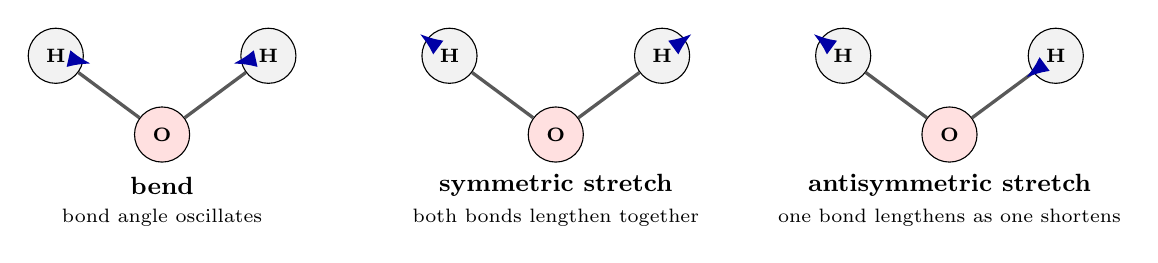
\begin{tikzpicture}[x=1cm,y=1cm,>=Latex,
 atom/.style={circle,draw,minimum size=7mm,font=\bfseries\scriptsize},
 move/.style={->,very thick,blue!65!black},
 bond/.style={line width=1.2pt,black!65}]
\begin{scope}[shift={(0,0)}]
 \node[atom,fill=red!12] (O) at (0,0) {O};
 \node[atom,fill=gray!10] (H1) at (-1.35,1.0) {H};
 \node[atom,fill=gray!10] (H2) at (1.35,1.0) {H};
 \draw[bond] (O)--(H1); \draw[bond] (O)--(H2);
 \draw[move] (H1) -- ++(0.45,-0.10);
 \draw[move] (H2) -- ++(-0.45,-0.10);
 \node[font=\small\bfseries] at (0,-0.65) {bend};
 \node[font=\scriptsize,align=center] at (0,-1.05) {bond angle oscillates};
\end{scope}
\begin{scope}[shift={(5.0,0)}]
 \node[atom,fill=red!12] (O) at (0,0) {O};
 \node[atom,fill=gray!10] (H1) at (-1.35,1.0) {H};
 \node[atom,fill=gray!10] (H2) at (1.35,1.0) {H};
 \draw[bond] (O)--(H1); \draw[bond] (O)--(H2);
 \draw[move] (H1) -- ++(-0.38,0.28);
 \draw[move] (H2) -- ++(0.38,0.28);
 \node[font=\small\bfseries] at (0,-0.65) {symmetric stretch};
 \node[font=\scriptsize,align=center] at (0,-1.05) {both bonds lengthen together};
\end{scope}
\begin{scope}[shift={(10.0,0)}]
 \node[atom,fill=red!12] (O) at (0,0) {O};
 \node[atom,fill=gray!10] (H1) at (-1.35,1.0) {H};
 \node[atom,fill=gray!10] (H2) at (1.35,1.0) {H};
 \draw[bond] (O)--(H1); \draw[bond] (O)--(H2);
 \draw[move] (H1) -- ++(-0.38,0.28);
 \draw[move] (H2) -- ++(-0.38,-0.28);
 \node[font=\small\bfseries] at (0,-0.65) {antisymmetric stretch};
 \node[font=\scriptsize,align=center] at (0,-1.05) {one bond lengthens as one shortens};
\end{scope}
\end{tikzpicture}
\caption{Schematic internal-coordinate character of the three retained water
normal modes.  The actual mass-weighted eigenvectors also move the oxygen atom
so that each mode is orthogonal to translation and rotation.  Arrows show
qualitative phase, not normalized displacement magnitude.}
\label{fig:modes}
\end{figure*}

\subsection*{Quantization of one normal mode}

\mathderiv In mass-weighted coordinates, the harmonic nuclear Hamiltonian is
\begin{equation}
\hat H_{\rm harm}=\sum_\mu\left(
\frac{\hat P_\mu^2}{2}+\frac{\omega_\mu^2\hat Q_\mu^2}{2}\right),
\qquad [\hat Q_\mu,\hat P_\nu]=i\delta_{\mu\nu}.
\label{eq:harmonic-hamiltonian}
\end{equation}
Define bosonic creation and annihilation operators by
\begin{align}
\hat Q_\mu&=\frac{\hat b_\mu^\dagger+\hat b_\mu}
{\sqrt{2\omega_\mu}},
&
\hat P_\mu&=i\sqrt{\frac{\omega_\mu}{2}}
(\hat b_\mu^\dagger-\hat b_\mu),
\label{eq:qp-boson}\\
[\hat b_\mu,\hat b_\nu^\dagger]&=\delta_{\mu\nu},
&
\hat n_\mu&=\hat b_\mu^\dagger\hat b_\mu.
\end{align}
Their action on harmonic-oscillator states is
\begin{equation}
\hat b_\mu\ket{n_\mu}=\sqrt{n_\mu}\ket{n_\mu-1},
\qquad
\hat b_\mu^\dagger\ket{n_\mu}
=\sqrt{n_\mu+1}\ket{n_\mu+1}.
\label{eq:ladder-action}
\end{equation}
Substituting Eq.~\eqref{eq:qp-boson} into the quadratic kinetic and potential
terms, and using
$\hat b_\mu\hat b_\mu^\dagger=\hat b_\mu^\dagger\hat b_\mu+1$, gives
\begin{equation}
\hat H_{\rm harm}=\sum_\mu\omega_\mu
\left(\hat n_\mu+\frac12\right).
\label{eq:harmonic-number}
\end{equation}
The eigenvalue of $\hat n_\mu$ is the number of vibrational quanta in mode
$\mu$.  The bend is the softest retained coordinate, so it has the smallest
curvature and frequency.  Stretching an O--H bond is stiffer, which places both
stretch modes above the bend; the antisymmetric stretch is slightly higher
than the symmetric stretch in this RHF/STO-3G calculation.  A crystal extends
the same bosonic algebra to delocalized modes carrying crystal momentum.  An
isolated water molecule instead has three discrete internal modes.

\physical The zero-point energy of the three uncoupled modes is
\begin{equation}
E_{\rm ZPE}=\frac12\sum_\mu\omega_\mu.
\label{eq:zpe}
\end{equation}
This positive energy remains even when every occupation number is zero,
because the uncertainty relation prevents a harmonic coordinate and its
conjugate momentum from both having zero variance.

\conceptbreak

\section*{Part IV. Active-space many-electron Hamiltonian}

\subsection*{Why an active space is introduced}

\micro The oxygen $1s$ core is chemically inert at the energy scale of the
retained valence vibrations.  Freezing it reduces the correlated problem while
preserving its mean-field contribution in the effective coefficients.

\mathderiv STO-3G gives seven spatial molecular orbitals for H$_2$O.  The
lowest orbital, dominated by O $1s$, is constrained to remain doubly occupied.
The remaining eight electrons occupy six active spatial orbitals.  This is
CAS$(8e,6o)$, with
\begin{equation}
\begin{gathered}
N_{\rm orb}=6,\qquad N_\alpha=N_\beta=4,\\
\dim\mathcal H_{\rm el}=\binom64\binom64=225.
\end{gathered}
\label{eq:cas-dimension}
\end{equation}
The active-space electronic Hamiltonian at the center geometry is
\begin{align}
\hat H_{\rm el}^{(0)}={}&E_{\rm sc}^{(0)}
+\sum_{pq=1}^{6}\sum_{\sigma\in\{\alpha,\beta\}}
h_{pq}^{(0)}a_{p\sigma}^\dagger a_{q\sigma}\nonumber\\
&+\frac12\sum_{pqrs=1}^{6}\sum_{\sigma\tau}
(pr|qs)^{(0)}
a_{p\sigma}^\dagger a_{q\tau}^\dagger
a_{s\tau}a_{r\sigma}.
\label{eq:active-hamiltonian}
\end{align}
The operator $a_{p\sigma}^\dagger$ creates an electron in spatial orbital $p$
with spin $\sigma$, and $a_{p\sigma}$ annihilates it.  They satisfy
\begin{equation}
\{a_{p\sigma},a_{q\tau}^\dagger\}=\delta_{pq}\delta_{\sigma\tau},
\qquad
\{a_{p\sigma},a_{q\tau}\}=0.
\label{eq:fermion-algebra}
\end{equation}
The scalar $E_{\rm sc}^{(0)}$ contains nuclear repulsion and the frozen-core
contraction.  The coefficient $h_{pq}^{(0)}$ is an effective one-electron
integral in the center MO basis.  The coefficient
\begin{equation}
(pr|qs)=\iint \phi_p^*(1)\phi_r(1)\frac1{r_{12}}
\phi_q^*(2)\phi_s(2)\,d1d2
\label{eq:mo-eri}
\end{equation}
is a two-electron Coulomb integral in the index convention used by the stored
Hamiltonian.

\commentaryblock Each one-body term moves one electron between orbitals.  Each
two-body term simultaneously annihilates two occupied spin orbitals and
creates two spin orbitals.  The second-quantized form compactly enforces
particle indistinguishability and fermionic antisymmetry.

\subsection*{Integral transformation and frozen-core contraction}

\micro The active Hamiltonian is obtained by changing the AO tensor basis to
the converged MO basis and then analytically contracting the doubly occupied
core orbital.

\mathderiv The AO-to-MO transformations are
\begin{align}
h_{pq}&=\sum_{\mu\nu}C_{\mu p}C_{\nu q}h^{\rm core}_{\mu\nu},\nonumber\\
(pr|qs)&=\sum_{\mu\nu\lambda\kappa}
C_{\mu p}C_{\nu r}C_{\lambda q}C_{\kappa s}
(\mu\nu|\lambda\kappa).
\label{eq:ao-mo-transform}
\end{align}
Let $i,j$ label frozen doubly occupied core orbitals and $p,q$ active orbitals.
Their mean-field contribution becomes
\begin{align}
E_{\rm core}
={}&V_{NN}+2\sum_i h_{ii}
+\sum_{ij}\left[2(ii|jj)-(ij|ji)\right],\nonumber\\
h^{\rm act}_{pq}
={}&h_{pq}
+\sum_i\left[2(pq|ii)-(pi|iq)\right].
\label{eq:frozen-core}
\end{align}
The first line is absorbed into $E_{\rm sc}^{(0)}$; the second modifies the
active one-electron coefficients.  The active two-electron integrals retain
their MO-transformed values.

\commentaryblock Freezing a core orbital is an exact contraction within the
declared approximation that its occupation remains two.  Its Coulomb and
exchange fields continue to act on every active electron through
$h^{\rm act}$.  The approximation removes configurations containing a core
hole or an electron promoted from the core into an active or external orbital.

\subsection*{Classical configuration interaction}

\mathderiv Let $\{\ket I\}$ be every Slater determinant with four alpha and
four beta electrons distributed among the six active spatial orbitals.  Expand
\begin{equation}
\ket{\Psi_{\rm CAS}}=\sum_I c_I\ket I,\qquad
\sum_I|c_I|^2=1.
\label{eq:ci-expansion}
\end{equation}
Projection of the Schrodinger equation onto determinant $\bra I$ gives the
matrix eigenproblem
\begin{equation}
\sum_J H_{IJ}c_J=E_{\rm CAS}^{\rm el}c_I,\qquad
H_{IJ}=\bra I\hat H_{\rm el}^{(0)}\ket J.
\label{eq:ci-eigenproblem}
\end{equation}
The Slater--Condon rules evaluate $H_{IJ}$ from the one- and two-electron
integrals.  Since the Hamiltonian contains at most two-body operators,
$H_{IJ}$ vanishes when determinants $I$ and $J$ differ by more than two
spin-orbital occupations.  This selection rule makes the configuration matrix
sparse even before symmetry is used.

\physical The RHF determinant supplies one electronic configuration.  The CAS
eigenvector superposes every allowed valence configuration, thereby permitting
electrons to avoid one another through correlated occupation amplitudes.  The
correlation lowering
\begin{equation}
E_{\rm corr}=E_{\rm CAS}^{\rm el}-E_{\rm RHF}<0
\label{eq:correlation-energy}
\end{equation}
belongs to this fixed RHF-derived orbital basis and active space.  A CASSCF
calculation adds orbital optimization to the configuration-interaction
optimization, so its geometry, Hessian, and displaced-orbital response would
form a different and more internally correlated electronic surface.

\conceptbreak

\section*{Part V. Constructing vibronic coefficients}

\subsection*{Linear response along a normal coordinate}

\micro The vibronic model asks how every electronic coefficient changes when
the nuclei move infinitesimally along one normal mode.

\mathderiv Express the electronic Hamiltonian in the center MO frame and expand
it about $Q_\mu=0$:
\begin{align}
\hat H_{\rm el}(\mathbf Q)
={}&\hat H_{\rm el}^{(0)}
+\sum_{\mu\in\mathcal M}\hat D_\mu Q_\mu+O(Q^2),\nonumber\\
\hat D_\mu
={}&\left.\frac{\partial\hat H_{\rm el}}
{\partial Q_\mu}\right|_{\mathbf Q=0}.
\label{eq:linear-expansion}
\end{align}
The retained mode set is
\begin{equation}
\mathcal M=\{\mathrm{bend},\mathrm{symmetric\ stretch},
\mathrm{antisymmetric\ stretch}\}.
\end{equation}
Differentiating Eq.~\eqref{eq:active-hamiltonian} gives
\begin{align}
\hat D_\mu={}&E'_\mu
+\sum_{pq\sigma}h'_{\mu,pq}a_{p\sigma}^\dagger a_{q\sigma}\nonumber\\
&+\frac12\sum_{pqrs\sigma\tau}g'_{\mu,prqs}
a_{p\sigma}^\dagger a_{q\tau}^\dagger a_{s\tau}a_{r\sigma},
\label{eq:derivative-operator}
\end{align}
where
\begin{equation}
E'_\mu=\left.\frac{\partial E_{\rm sc}}{\partial Q_\mu}\right|_0,
\quad
h'_{\mu,pq}=\left.\frac{\partial h_{pq}}{\partial Q_\mu}\right|_0,
\quad
g'_{\mu,prqs}=\left.\frac{\partial(pr|qs)}{\partial Q_\mu}\right|_0.
\label{eq:coefficient-derivatives}
\end{equation}

\physical The scalar derivative changes the frozen-core and nuclear part of
the energy.  The one-body derivative changes orbital energies and one-electron
mixing.  The two-body derivative changes electron--electron interaction
matrix elements.  A complete first derivative contains all three pieces.

\subsection*{Centered finite differences and orbital alignment}

\micro A centered difference isolates the odd, linear response by canceling
the equilibrium value and every even power of the displacement.

\mathderiv Let $A(Q)$ denote any scalar or tensor coefficient.  Taylor
expansion at the two displaced geometries gives
\begin{align}
A(+\delta Q)
&=A_0+\delta Q\,A'_0+\frac{\delta Q^2}{2}A''_0
+\frac{\delta Q^3}{6}A'''_0+O(\delta Q^4),\nonumber\\
A(-\delta Q)
&=A_0-\delta Q\,A'_0+\frac{\delta Q^2}{2}A''_0
-\frac{\delta Q^3}{6}A'''_0+O(\delta Q^4).
\label{eq:fd-taylor}
\end{align}
Subtracting and dividing by $2\delta Q$ yields
\begin{equation}
\frac{A(+\delta Q)-A(-\delta Q)}{2\delta Q}
=A'_0+\frac{\delta Q^2}{6}A'''_0+O(\delta Q^4).
\label{eq:fd-error}
\end{equation}
The leading truncation error is therefore quadratic in the step.  Applying
this identity to the Psi4 coefficients gives
\begin{align}
E'_\mu&\approx\frac{E_{\rm sc}(+\delta Q_\mu)-E_{\rm sc}(-\delta Q_\mu)}
{2\delta Q_\mu},\nonumber\\
h'_{\mu,pq}&\approx\frac{h_{pq}(+\delta Q_\mu)-h_{pq}(-\delta Q_\mu)}
{2\delta Q_\mu},
\label{eq:fd-one}\\
g'_{\mu,prqs}&\approx\frac{g_{prqs}(+\delta Q_\mu)-g_{prqs}(-\delta Q_\mu)}
{2\delta Q_\mu}.
\label{eq:fd-two}
\end{align}
The calculation uses a primary displacement and repeats the construction at
half that displacement.  Agreement tests whether the derivative has entered
the quadratic-error regime predicted by Eq.~\eqref{eq:fd-error}.

Molecular orbitals possess a gauge freedom: an orbital may change sign, and
orbitals inside a nearly degenerate subspace may rotate, without changing the
SCF determinant.  Direct subtraction of independently canonicalized MO
tensors can therefore confuse gauge motion with physical nuclear response.
Let $S^{0\pm}_{pq}=\langle\phi_p(0)|\phi_q(\pm\delta Q)\rangle$.  An orthogonal
Procrustes alignment chooses a rotation $U_\pm$ that maximizes
\begin{equation}
\Tr(U_\pm^{\mathsf T}S^{0\pm}),
\qquad
S^{0\pm}=V\Sigma W^{\mathsf T},
\qquad U_\pm=VW^{\mathsf T}.
\label{eq:procrustes}
\end{equation}
The displaced one- and two-electron tensors are transformed by $U_\pm$ before
Eqs.~\eqref{eq:fd-one}--\eqref{eq:fd-two} are applied.

\impl This alignment is the bridge between chemistry and numerics.  It makes
the derivative tensors refer to one fixed set of active orbitals, so the
operator $\hat D_\mu$ describes a change of coefficients in a common Fock
space.

\begin{table}[ht]
\centering
\caption{Qualitative structure of the retained electronic response.}
\scriptsize
\begin{tabular}{@{}p{0.30\columnwidth}p{0.22\columnwidth}
  p{0.16\columnwidth}p{0.16\columnwidth}@{}}
\toprule
Mode & scalar & one-body & two-body\\\midrule
Bend & active & active & active\\
Symmetric stretch & active & active & active\\
Antisymmetric stretch & symmetry-suppressed & active & active\\
\bottomrule
\end{tabular}
\label{tab:derivative-structure}
\end{table}

\commentaryblock The antisymmetric scalar derivative is suppressed by the
center symmetry, yet its one- and two-body derivative tensors are substantial.
The mode can therefore rearrange electronic matrix elements even when the
scalar contribution has zero first derivative.

\subsection*{The vibration-modulated two-electron interaction}

\mathderiv Substituting the quantized coordinate from
Eq.~\eqref{eq:qp-boson} into the two-body piece of
$\hat D_\mu\hat Q_\mu$ gives
\begin{equation}
\boxed{
\frac{1}{2\sqrt{2\omega_\mu}}
\sum_{pqrs\sigma\tau}g'_{\mu,prqs}
a_{p\sigma}^\dagger a_{q\tau}^\dagger
(b_\mu^\dagger+b_\mu)a_{s\tau}a_{r\sigma}.}
\label{eq:advisor-term}
\end{equation}
This is the $a^\dagger a^\dagger b a a$ family of terms: a two-electron
scattering amplitude is modulated by creation or annihilation of one
vibrational quantum.  Fermionic and bosonic operators commute because they act
on different tensor factors, so the boson factor may be written between the
creation and annihilation operators as in Eq.~\eqref{eq:advisor-term}.

\materials In crystalline electron--phonon theory, a normal displacement
modulates band energies, hopping amplitudes, and screened electron--electron
interactions.  Equation~\eqref{eq:advisor-term} is the finite-molecule,
active-orbital analogue of that response.  Its mode label replaces crystal
momentum, and its derivative integral $g'_\mu$ records how Coulomb scattering
changes under the collective nuclear displacement \cite{Giustino}.

\conceptbreak

\section*{Part VI. The complete molecular-vibronic model}

\mathderiv Combining the equilibrium electronic Hamiltonian, three harmonic
oscillators, and the linear response gives
\begin{equation}
\boxed{
\hat H_{\rm H_2O}^{\rm lin}=\hat H_{\rm el}^{(0)}
+\sum_{\mu\in\mathcal M}\omega_\mu\left(\hat n_\mu+\frac12\right)
+\sum_{\mu\in\mathcal M}\hat D_\mu\hat Q_\mu.}
\label{eq:full-vibronic}
\end{equation}
Every symbol in Eq.~\eqref{eq:full-vibronic} has now been constructed:
$\hat H_{\rm el}^{(0)}$ is Eq.~\eqref{eq:active-hamiltonian}; $\omega_\mu$ and
the coordinate convention come from Eqs.~\eqref{eq:normal-eigenproblem} and
\eqref{eq:qp-boson}; $\hat n_\mu$ counts quanta; and $\hat D_\mu$ is the full
scalar, one-body, and two-body derivative in
Eq.~\eqref{eq:derivative-operator}.

\physical The harmonic term penalizes nuclear displacement from equilibrium.
The linear coupling allows the electronic state and oscillator wavefunction to
relax together.  The ground state is therefore generally entangled:
\begin{equation}
\ket{\Psi_0}=\sum_{I,n_b,n_s,n_a}
C_{I,n_b,n_s,n_a}\ket{I}_{\rm el}
\ket{n_b,n_s,n_a}_{\rm vib},
\label{eq:entangled-state}
\end{equation}
where $I$ labels electronic configurations and $(n_b,n_s,n_a)$ label bend,
symmetric-stretch, and antisymmetric-stretch occupations.  An electronic
configuration can favor a displaced oscillator distribution, and that
distribution feeds back on electronic mixing.

\subsection*{What the linear model retains}

The model retains harmonic nuclear curvature and first electronic response.
Its first omitted terms are
\begin{equation}
\frac12\sum_{\mu\nu}\hat D^{(2)}_{\mu\nu}Q_\mu Q_\nu,
\qquad
\sum_{\mu\nu\lambda}\Phi_{\mu\nu\lambda}Q_\mu Q_\nu Q_\lambda,
\label{eq:omitted-terms}
\end{equation}
where $\hat D^{(2)}_{\mu\nu}$ is a quadratic electronic response and
$\Phi_{\mu\nu\lambda}$ is an anharmonic force constant.  Diagonal quadratic
terms change mode curvature; off-diagonal terms couple modes; cubic and higher
terms generate anharmonicity.  Their omission defines the scientific boundary
of the present Hamiltonian.

\commentaryblock ``Molecular vibronic'' here means that electronic and
vibrational degrees of freedom coexist in one Hamiltonian and interact through
mode-dependent electronic derivatives.  Its domain is a local, linearized
potential-energy surface represented in a finite orbital and oscillator basis;
convergence studies determine how closely that domain approximates physical
water.

\conceptbreak

\section*{Part VII. Classical solution of the coupled Hamiltonian}

\subsection*{The direct-product basis}

\micro The classical calculation turns the operator in
Eq.~\eqref{eq:full-vibronic} into a sparse matrix.  Its rows and columns are
labelled by an electronic determinant and by the occupation of each normal
mode.

\mathderiv Let $I$ index the CAS determinants introduced in
Eq.~\eqref{eq:ci-expansion}.  For selected mode cutoffs $n_{\mu,\max}$, define
the direct-product basis
\begin{equation}
\mathcal B=\left\{
\ket{I}\otimes\ket{n_b,n_s,n_a}:
0\le n_\mu\le n_{\mu,\max}
\right\}.
\label{eq:direct-product-basis}
\end{equation}
Its dimension follows directly from independent choices of electron
configurations and oscillator occupations:
\begin{equation}
\dim\mathcal B=\binom64^2
\prod_{\mu\in\mathcal M}(n_{\mu,\max}+1).
\label{eq:coupled-dimension}
\end{equation}
For the compact cutoff $(1,1,1)$, the $225$ electronic configurations combine
with $2^3$ vibrational occupations to produce an $1800$-dimensional classical
matrix problem.  This count is useful because it predicts memory, matrix-vector
cost, and the growth caused by increasing a vibrational cutoff.

The matrix elements are
\begin{equation}
H_{I\mathbf n,J\mathbf m}
=\bra{I,\mathbf n}\hat H_{\rm H_2O}^{\rm lin}
\ket{J,\mathbf m}.
\label{eq:coupled-matrix-elements}
\end{equation}
The equilibrium electronic Hamiltonian preserves every vibrational
occupation, and the harmonic term is diagonal in both $I$ and $\mathbf n$.
The coordinate matrix element
\begin{equation}
\bra{n'_mu}\hat Q_\mu\ket{n_\mu}
=\frac{\sqrt{n_\mu+1}\,\delta_{n'_mu,n_\mu+1}
+\sqrt{n_\mu}\,\delta_{n'_mu,n_\mu-1}}
{\sqrt{2\omega_\mu}}
\label{eq:q-matrix-element}
\end{equation}
shows that a linear vibronic term changes exactly one mode occupation by one
quantum.  The scalar part of $\hat D_\mu$ leaves $I$ unchanged, its one-body
part connects determinants differing by one spin orbital, and its two-body
part connects determinants differing by at most two spin orbitals.  These
selection rules create a highly structured sparse matrix.

\commentaryblock Matrix sparsity has a physical meaning.  The Hamiltonian
implements local moves in configuration space: one vibrational quantum is
created or removed while zero, one, or two electronic occupations change.
Most arbitrary pairs of basis states cannot be connected by a single
Hamiltonian application, so their matrix element is exactly zero.

\subsection*{Lanczos and Krylov-space diagonalization}

\micro The ground-state calculation needs the lowest eigenpair, rather than
every excited eigenvector.  A Krylov method extracts that information through
repeated sparse matrix-vector products.

\mathderiv Starting from a normalized trial vector $v_1$, an $m$-dimensional
Krylov subspace is
\begin{equation}
\mathcal K_m(H,v_1)=\Span\{v_1,Hv_1,H^2v_1,\ldots,H^{m-1}v_1\}.
\label{eq:krylov-space}
\end{equation}
Lanczos orthogonalization produces the basis matrix
$V_m=[v_1,\ldots,v_m]$ and the small tridiagonal projection
\begin{equation}
T_m=V_m^\dagger H V_m.
\label{eq:lanczos-projection}
\end{equation}
The smallest eigenpair $(\theta_0,y_0)$ of $T_m$ gives the Ritz approximation
\begin{equation}
E_0\approx\theta_0,
\qquad
\ket{\Psi_0}\approx V_my_0.
\label{eq:ritz-pair}
\end{equation}
The residual
\begin{equation}
r_0=H(V_my_0)-\theta_0(V_my_0)
\label{eq:eigensolver-residual}
\end{equation}
measures numerical convergence.  Sparse storage and matrix-vector products
avoid the memory cost of dense diagonalization while preserving the exact
matrix elements of the declared finite model.

\physical The resulting $E_0$ is the lowest energy permitted by the chosen
orbital basis, frozen-core active space, linear vibronic expansion, and
vibrational cutoffs.  Within those choices, the eigensolver error can be driven
below the model errors.  Improving the physical prediction then requires a
larger basis or a richer Hamiltonian, rather than a different diagonalization
strategy.

\subsection*{Reading the energy balance}

Define the uncoupled product baseline and coupling relaxation by
\begin{align}
E_{\rm uncoupled}&=E_{\rm CAS}^{\rm el}+E_{\rm ZPE},\nonumber\\
\Delta E_{\rm vib}&=E_0-E_{\rm uncoupled}.
\label{eq:energy-balance}
\end{align}
The zero-point term raises the energy above the clamped-nuclei electronic
minimum.  The coupled wavefunction then lowers the product-state baseline by
allowing electronic configurations and vibrational occupations to reorganize
together, so $\Delta E_{\rm vib}<0$.  In the current compact fixture, the
coupling recovers roughly one third of the zero-point increase.  The remaining
net shift is positive.  This ratio communicates the competition between two
mechanisms more clearly than the absolute molecular energy, whose large core
contribution is common to all three quantities.

\conceptbreak

\section*{Part VIII. Validation as materials computation}

\subsection*{Internal algebraic checks}

\begin{table}[ht]
\centering
\caption{What the principal internal checks establish.}
\scriptsize
\begin{tabular}{@{}p{0.30\columnwidth}p{0.62\columnwidth}@{}}
\toprule
Check & Interpretation\\\midrule
$h=h^\dagger$ & The one-electron operator gives real expectation values.\\
ERI permutation symmetry & Electron labels and integral-index conventions are consistent.\\
$H=H^\dagger$ & The assembled many-body Hamiltonian has a real spectrum.\\
RHF energy reconstruction & AO integrals, MO transformation, frozen core, and determinant occupations agree.\\
$L^{\mathsf T}L=I$ & Normal coordinates are mutually orthonormal.\\
Translation--rotation projection & Internal modes contain negligible rigid molecular motion.\\
Projected-gradient equality & Mass weighting, mode phase, orbital alignment, and all derivative pieces agree.\\
\bottomrule
\end{tabular}
\label{tab:checks}
\end{table}

These checks are identities implied by the mathematics rather than fits to a
desired answer.  A failure therefore localizes the implementation error.  For
example, a non-Hermitian $h$ points to tensor transformation or indexing;
incorrect ERI symmetry points to a four-index convention; and excessive
translation--rotation overlap points to mass weighting or mode projection.

The most comprehensive coefficient check compares the expectation of the full
derivative operator on the RHF determinant with the analytic Cartesian Psi4
gradient projected onto the same mode:
\begin{equation}
\langle\Phi_{\rm RHF}|\hat D_\mu|\Phi_{\rm RHF}\rangle
\stackrel{?}{=}L_\mu^{\mathsf T}M^{-1/2}\nabla_{\mathbf R}E_{\rm RHF}.
\label{eq:gradient-check}
\end{equation}
The retained calculation satisfies this equality within its configured
numerical tolerance for every mode.  One comparison simultaneously probes the
scalar, one-body, and two-body derivatives together with mode sign, orbital
alignment, and mass-weighting conventions.

\subsection*{Vibrational cutoff convergence}

Two complementary quantities test a vibrational cutoff.  The energy change
under enlargement is
\begin{equation}
\rho_E=\frac{|E_0^{\rm small}-E_0^{\rm large}|}
{\epsilon_E},
\label{eq:cutoff-energy-ratio}
\end{equation}
where $\epsilon_E$ is the declared energy tolerance.  The boundary diagnostic
is
\begin{equation}
w_{\partial}=\sum_{\mathbf n\in\partial\mathcal B}
\sum_I|C_{I\mathbf n}|^2,
\qquad
\rho_{\partial}=\frac{w_{\partial}}{\epsilon_{\partial}},
\label{eq:boundary-weight}
\end{equation}
where $\partial\mathcal B$ contains states that occupy at least one highest
retained oscillator level.  The current comparison gives $\rho_E\approx2.15$
and $\rho_{\partial}\approx14.7$.  Both ratios exceed unity, so $(1,1,1)$ is a
compact working representation rather than a converged vibrational basis.
The larger boundary ratio also shows why an apparently modest energy change
cannot by itself establish wavefunction convergence.

\materials A cutoff study plays the same epistemic role as a plane-wave cutoff
study in a crystal calculation: it asks whether enlarging the numerical
representation changes the observable beyond the declared tolerance.  The
representation differs, yet the convergence logic is identical.

\begin{figure*}[t]
\centering
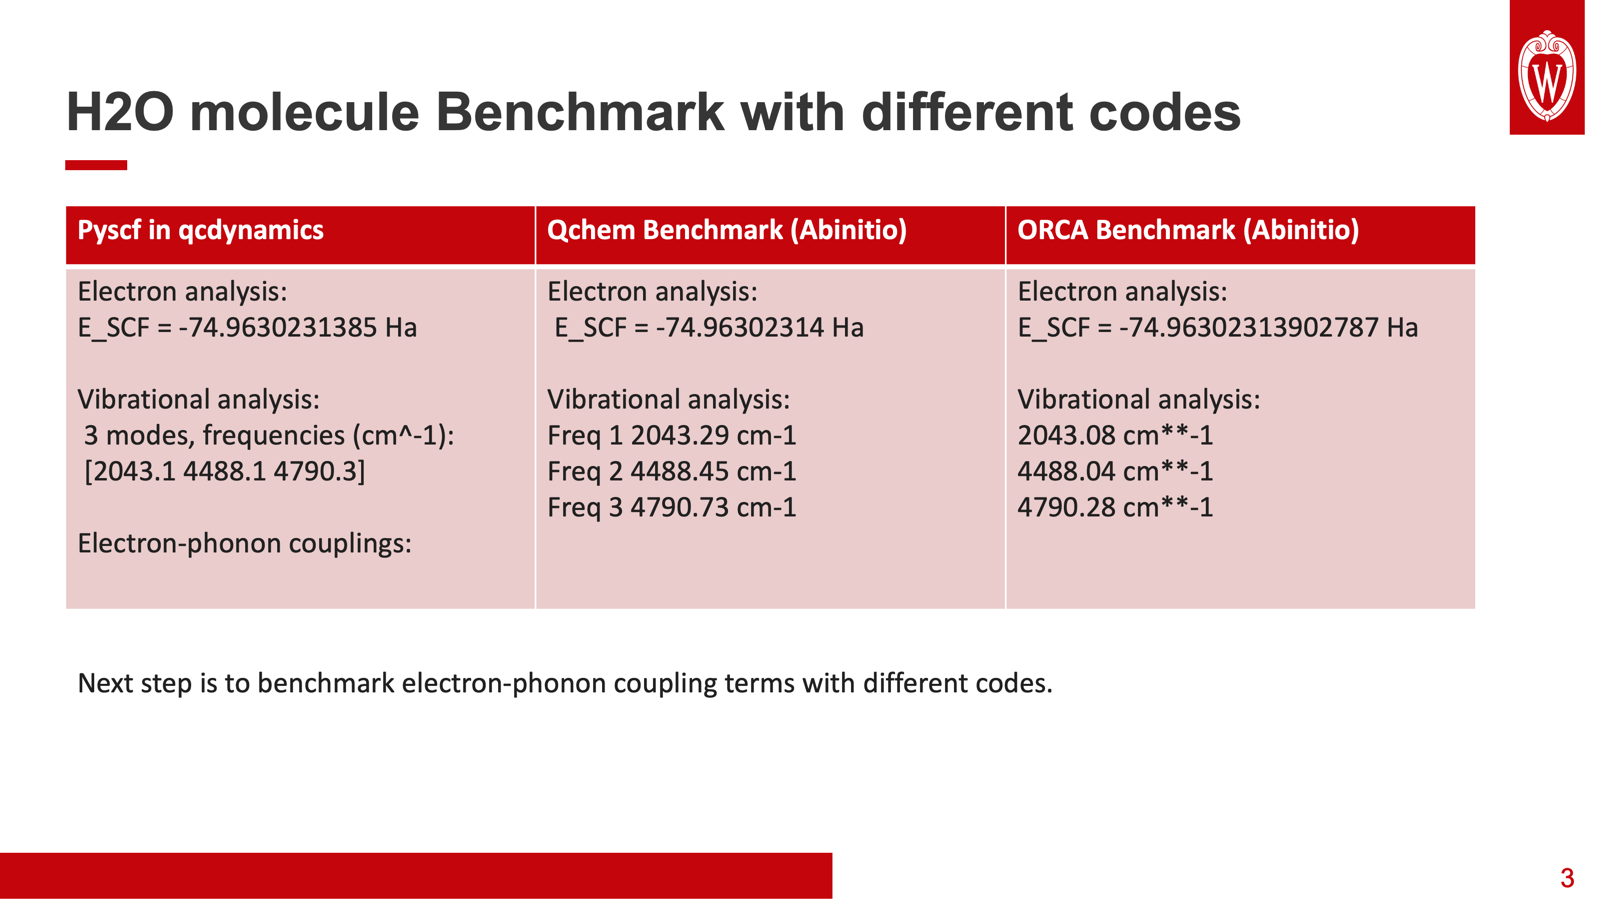
\includegraphics[width=0.94\textwidth]{../assets/h2o_cross_code_benchmark_colleague_20260714.png}
\caption{Collaborator-supplied cross-code H$_2$O benchmark.  The three rows
agree tightly for the collaborator's input.  The slide does not record its
geometry, basis, isotope masses, Hessian projection convention, or convergence
thresholds, so matching the visible numbers required reconstruction of the
geometry condition.}
\label{fig:cross-code}
\end{figure*}

The slide is most useful as a lesson in controlled comparison.  Three programs
agree when they solve the same stated problem.  Our retained optimized-geometry
calculation initially appeared different because it solved the RHF/STO-3G
problem at a different nuclear geometry.  Repeating Psi4 and PySCF at identical
optimized coordinates produces numerical agreement in both the SCF energy and
the three Hessian frequencies.  Repeating the calculation at the fixed,
near-experimental geometry reproduces the pattern in the slide.  Geometry,
rather than program identity, explains the apparent disagreement.

This comparison validates the center electronic calculation and harmonic
analysis under matched inputs.  A complete cross-code validation of the
vibronic Hamiltonian requires the next layer: compare aligned scalar,
one-electron, and two-electron derivatives after fixing geometry, basis,
masses, mode phases, active orbitals, and orbital gauge.

\begin{table*}[t]
\centering
\caption{Scope of the current cross-code evidence.}
\small
\begin{tabular}{@{}p{0.21\textwidth}p{0.23\textwidth}p{0.47\textwidth}@{}}
\toprule
Evidence object & Current result & Scientific scope\\\midrule
SCF energy at retained coordinates &
Agreement to numerical precision &
Confirms the matched-geometry center RHF/STO-3G energy across Psi4 and PySCF.\\
Three Hessian frequencies at retained coordinates &
Agreement to numerical precision &
Confirms matched masses, Hessian processing, and normal-mode eigenvalues.\\
Near-experimental fixed geometry &
Collaborator pattern recovered &
Explains the visible slide/fixture difference through geometry.\\
Mode-resolved coefficient derivatives &
Independent result pending &
Requires matched active orbitals, mode phase, orbital gauge, and comparison of
$E'_\mu$, $h'_\mu$, and $g'_\mu$.\\
\bottomrule
\end{tabular}
\end{table*}

\subsection*{A hierarchy of approximation and convergence}

\begin{enumerate}[leftmargin=1.35em,itemsep=2pt]
\item \textbf{Relativistic and Born--Oppenheimer model.}  The calculation uses
a nonrelativistic clamped-nuclei electronic surface.  Nonadiabatic derivative
couplings between distinct electronic surfaces enter at a richer model level.
\item \textbf{Electronic method.}  Geometry, Hessian, orbitals, and derivatives
are RHF-referenced.  Correlation is introduced later by exact solution of the
fixed CAS Hamiltonian.
\item \textbf{Orbital basis.}  STO-3G is minimal.  A basis ladder such as
double-zeta, polarization, and larger correlation-consistent bases is needed
for basis convergence.
\item \textbf{Active space.}  CAS$(8e,6o)$ freezes O $1s$ and omits external
virtual orbitals.  Active-orbital enlargement tests this approximation.
\item \textbf{Local vibronic expansion.}  The Hamiltonian is linear in $Q$ and
harmonic in nuclear motion.  Quadratic response and anharmonic force constants
define the next model tier.
\item \textbf{Finite difference and orbital gauge.}  The $0.1/0.05$ step check
and center-frame alignment control truncation and gauge errors.
\item \textbf{Vibrational basis.}  The current $(1,1,1)$ representation fails its
energy and boundary-weight tests against $(2,2,2)$.
\item \textbf{Ground-state solver.}  The Lanczos residual separates numerical
eigensolver convergence from errors in the finite Hamiltonian model.
\end{enumerate}

\subsection*{Relation to a periodic diamond workflow}

\begin{table}[ht]
\centering
\caption{Shared scientific tasks with system-specific representations.}
{\scriptsize
\begin{tabular}{@{}p{0.22\columnwidth}p{0.35\columnwidth}p{0.35\columnwidth}@{}}
\toprule
Task & Periodic diamond & Molecular H$_2$O\\\midrule
Electronic basis & plane waves plus pseudopotential & atom-centered Gaussian STO-3G\\
Boundary condition & periodic crystal & isolated finite molecule\\
Sampling & Brillouin-zone $k$ mesh & discrete molecular orbitals\\
Structure & lattice/EOS or cell relaxation & bond lengths, angle, molecular optimization\\
Curvature & crystal phonons, dynamical matrix & three molecular normal modes\\
Electronic response & electron--phonon matrix elements & $E'_\mu,h'_\mu,g'_\mu$\\
Convergence & cutoff, $k$ mesh, cell size & basis, active space, $\delta Q$, $n_{\max}$\\
Observable & bands, DOS, elastic data & energy, modes, vibronic ground state\\
\bottomrule
\end{tabular}}
\label{tab:diamond-water}
\end{table}

Bloch's theorem, reciprocal-lattice vectors, $k$-point integration, band
structure, density of states, and an equation of state belong to periodic
crystals.  They are absent from this isolated H$_2$O calculation.  The
transferable content is the first-principles chain: choose a microscopic
Hamiltonian, choose and converge a finite representation, optimize structure,
differentiate the energy surface, validate independent implementations, and
trace each reported property to its numerical assumptions.

\conceptbreak

\section*{Part IX. Reproducible computational recipe}

\begin{enumerate}[leftmargin=1.35em,itemsep=2pt]
\item \textbf{Declare the molecular problem.}  Specify neutral singlet
H$_2$O, isotope masses, atomic units, RHF, STO-3G, integral algorithm, and SCF
thresholds.  This declaration fixes the mathematical meaning of every later
energy and frequency.
\item \textbf{Build AO integrals.}  Evaluate $S$, $T$, $V$, and the
electron-repulsion tensor in contracted Gaussian functions.  Verify integral
symmetries before any nonlinear iteration.
\item \textbf{Solve SCF and optimize geometry.}  Iterate density and Fock
matrices to a stationary RHF solution at every trial geometry.  Use analytic
gradients and controlled nuclear steps until both force and displacement
criteria are satisfied.
\item \textbf{Compute harmonic modes.}  Evaluate the Cartesian Hessian at the
stationary geometry, mass weight it, project translations and rotations,
diagonalize the internal block, and assign bend and stretch characters.
\item \textbf{Transform to the active electronic problem.}  Rotate AO
integrals into the center MO basis, contract the doubly occupied O $1s$ core,
and assemble the CAS$(8e,6o)$ scalar, one-body, and two-body tensors.
\item \textbf{Solve the clamped-nuclei CAS problem.}  Enumerate determinants,
construct matrix elements with Slater--Condon rules, and diagonalize the sparse
CI matrix.  Compare the CAS and RHF states to quantify valence correlation.
\item \textbf{Differentiate along normal coordinates.}  Generate positive
and negative mass-weighted displacements at a primary and half step.  Converge
an RHF calculation and integral transformation at every displaced geometry.
\item \textbf{Align and difference.}  Align displaced orbitals to the center
frame, transform all coefficient tensors, and apply centered differences.
Compare the two step sizes and reconstruct the projected analytic gradient.
\item \textbf{Assemble the coupled matrix.}  Form the direct-product basis in
Eq.~\eqref{eq:direct-product-basis}, use Eq.~\eqref{eq:q-matrix-element} for
oscillator couplings, and store only nonzero matrix elements.
\item \textbf{Compute and converge the coupled ground state.}  Use a Lanczos
or equivalent sparse Hermitian eigensolver, verify its residual, inspect mode
occupations and boundary weight, and repeat with larger vibrational cutoffs.
\item \textbf{Climb the model hierarchy.}  Repeat at larger Gaussian bases,
larger active spaces, correlated geometries, and higher-order vibronic terms.
Change one approximation at a time so each energy or spectrum shift has a
clear cause.
\end{enumerate}

\impl The main chemistry construction is anchored in
\codepath{src/quantum/chemistry/generate_h2o_linear_fd_fixture.py} and
\codepath{src/quantum/chemistry/molecular_hamiltonian.py}.  The latter defines
the scalar, one-body, and two-body molecular Hamiltonian.  The fixture
generator obtains and aligns Psi4 tensors, constructs $\hat D_\mu$, assembles
the finite electronic--vibrational representation, and emits the manifest,
diagnostics, coefficients, and classical reference data.  The external audit record is
\codepath{output/molecular_vibronic_h2o/h2o_cross_code_reference_audit.json}.

\subsection*{The next scientifically strongest calculation}

The most direct next ladder has three controlled changes.  First, repeat the
coupled classical calculation at successively larger vibrational cutoffs until
both energy change and boundary weight pass their tolerances.  Second,
regenerate the geometry, Hessian, orbital frame, and derivatives consistently
at a correlated level such as CASSCF so the normal coordinates and electronic
response belong to the same stationary correlated surface.  Third, compare
mode-resolved derivative tensors across independent electronic-structure codes
after matching geometry, basis, masses, mode phases, active orbitals, and
orbital gauge.  These steps target representation error, electronic-structure
error, and implementation error separately.

\conceptbreak

\section*{Transfer and repair problems}

\begin{enumerate}[leftmargin=1.35em,itemsep=3pt]
\item Starting from $R_{\rm SCF}=FPS-SPF$, transform to an orthonormal basis
and explain why a vanishing residual means the occupied density and Fock
operator are stationary with respect to occupied--virtual rotations.
\item Suppose one displaced antisymmetric-stretch orbital flips sign.  Show
how an unaligned central difference can create an $O(1/\delta Q)$ spurious
matrix derivative, then explain how overlap alignment removes it.
\item Extend Eq.~\eqref{eq:linear-expansion} through quadratic order.  Identify
which terms change a single mode's frequency and which terms couple two modes.
\item Design a convergence ladder for Gaussian basis, active space,
finite-difference step, and vibrational cutoff.  Choose one observable for each
stage and explain why changing one approximation at a time is necessary for
causal interpretation.
\item Propose a cross-code derivative benchmark whose output is invariant to
mode sign and active-orbital gauge.  Specify the transformations and norms that
must be reported.
\end{enumerate}

\conceptbreak

\section*{Dimensional and notation audit}

Atomic units make energy, length, mass-weighted coordinate, and frequency
numerically compact, yet dimensions still organize the equations.
$\omega_\mu$ has energy units because $\hbar=1$.  The coordinate
$Q_\mu=(b^\dagger+b)/\sqrt{2\omega_\mu}$ has units $\omega^{-1/2}$ in the
mass-weighted convention.  Therefore $\hat D_\mu=\partial\hat H/\partial Q_\mu$
has energy per $Q$, and $\hat D_\mu Q_\mu$ has energy.  The coefficients
$E'_{\mu}$, $h'_{\mu,pq}$, and $g'_{\mu,prqs}$ share energy-per-$Q$ units.  The
indices $p,q,r,s$ always label the six active spatial MOs; $\sigma,\tau$ label
alpha or beta spin; $\mu$ labels one of three normal modes; and $A,B$ label
nuclei.  This separation prevents orbital, mode, and Cartesian indices from
being silently interchanged.

\section*{Takeaway}

The current H$_2$O path is a complete, auditable chain from microscopic
Coulomb Hamiltonian to a finite classical electronic--vibrational eigenproblem.
Psi4 supplies the RHF/STO-3G molecular surface, optimized geometry, analytic
derivatives, Hessian, orbitals, and integral tensors.  Mass weighting supplies
three internal normal coordinates.  Frozen-core contraction and CAS
configuration interaction supply the correlated valence problem.  Aligned
finite differences supply scalar, one-electron, and two-electron vibronic
response, including vibration-modulated electron--electron scattering.
Finally, a sparse direct-product matrix and Lanczos eigensolve supply the
coupled molecular ground state of the declared finite model.

The central computational lesson is that ``the H$_2$O energy'' is never one
context-free number.  It belongs to a geometry, Gaussian basis, electronic
method, active space, normal-coordinate convention, vibronic expansion, and
vibrational cutoff.  Internal identities test the implementation; matched-
input cross-code calculations test reproducibility; and systematic enlargement
tests the physical approximations.  The present model passes its internal and
matched-geometry center checks while identifying three concrete upgrades: a
larger orbital basis, a correlated stationary surface with an independent
derivative audit, and a converged vibrational occupation basis.

\begin{thebibliography}{9}
\bibitem{BornOppenheimer}
M. Born and R. Oppenheimer, ``Zur Quantentheorie der Molekeln,''
\emph{Ann. Phys.} \textbf{389}, 457--484 (1927).

\bibitem{Roothaan}
C. C. J. Roothaan, ``New Developments in Molecular Orbital Theory,''
\emph{Rev. Mod. Phys.} \textbf{23}, 69--89 (1951).

\bibitem{STO3G}
W. J. Hehre, R. F. Stewart, and J. A. Pople, ``Self-Consistent Molecular-
Orbital Methods. I. Use of Gaussian Expansions of Slater-Type Atomic
Orbitals,'' \emph{J. Chem. Phys.} \textbf{51}, 2657--2664 (1969).

\bibitem{SzaboOstlund}
A. Szabo and N. S. Ostlund, \emph{Modern Quantum Chemistry: Introduction to
Advanced Electronic Structure Theory} (Dover, 1996).

\bibitem{Wilson}
E. B. Wilson, J. C. Decius, and P. C. Cross, \emph{Molecular Vibrations}
(McGraw--Hill, 1955).

\bibitem{Psi4}
D. G. A. Smith \emph{et al.}, ``Psi4 1.4: Open-source software for high-
throughput quantum chemistry,'' \emph{J. Chem. Phys.} \textbf{152}, 184108
(2020).

\bibitem{Giustino}
F. Giustino, ``Electron-phonon interactions from first principles,''
\emph{Rev. Mod. Phys.} \textbf{89}, 015003 (2017).

\end{thebibliography}

\end{document}
